\documentclass[letter,11pt]{article}

\usepackage[spanish,es-nodecimaldot]{babel}
\usepackage[utf8]{inputenc}

\usepackage{lmodern}
\usepackage[T1]{fontenc}
\usepackage{textcomp}

\usepackage{framed}
\usepackage[svgnames]{xcolor}
\colorlet{shadecolor}{Gainsboro!50}

\usepackage[shortlabels]{enumitem}
\usepackage{graphicx}
\usepackage{pstricks}

\usepackage{anysize}
\marginsize{3cm}{2cm}{2cm}{3cm}

\usepackage{siunitx}
\usepackage{amsmath}
\usepackage{array}

\usepackage{fancyhdr}
\usepackage{lastpage}
\pagestyle{fancy}
\fancyhf{}
\fancyhead[LE,RO]{Física Básica II}
\fancyfoot[CO,CE]{\thepage\ de \pageref{LastPage}}

\special{papersize=215.9mm,279.4mm}

\usepackage[
    pdfauthor={Carlos Eduardo Caballero Burgoa},%
    pdftitle={Física Básica II},%
    pdfsubject={Tarea 24},%
    colorlinks,%
    citecolor=black,%
    filecolor=black,%
    linkcolor=black,%
    urlcolor=black,
    breaklinks]{hyperref}
\usepackage{breakurl}

\newcommand{\blankpage}{
\newpage
\thispagestyle{empty}
\mbox{}
\newpage
}

\renewcommand{\arraystretch}{1.2}

\begin{document}

\begin{center}
    {\Large \bf{Tarea \#24}}
\end{center}

Una partícula de masa igual a $3\, [kg]$ se mueve a lo largo del eje $x$ atraída
hacia el origen por una fuerza cuya magnitud es numéricamente igual a $12x$. La
partícula también se somete a una fuerza de amortiguación cuya magnitud es
numéricamente igual a $12$ veces la velocidad instantánea. Si inicialmente está
en reposo en $x = 10\, [m]$.

\begin{enumerate}[a)]
    \item Encuentre la posición en función del tiempo.
    \item Encuentre la velocidad en función del tiempo.
\end{enumerate}

\vspace{0.5cm}
\textbf{Solución:} \\

\begin{figure}[!h]
\centering
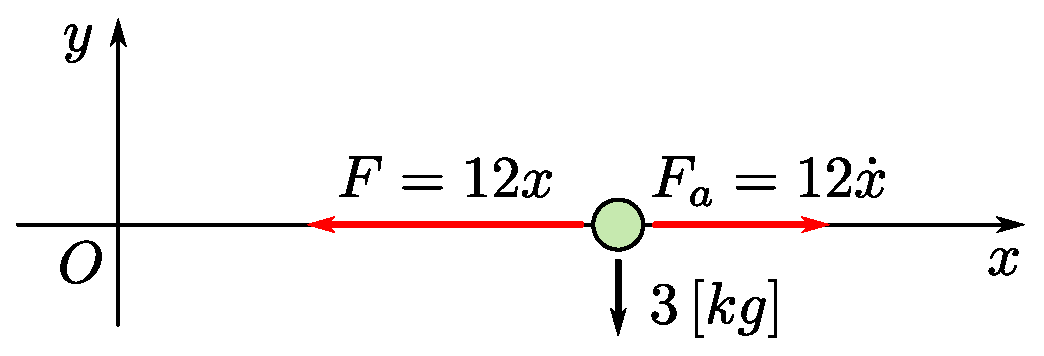
\includegraphics[scale=0.40]{resources/f1.eps}
\end{figure}

Considerando la segunda ley de \emph{Newton}:

\begin{equation*}
    \sum F = m\, a
\end{equation*}
\begin{equation*}
    - F - F_a = m\, a
\end{equation*}
\begin{equation*}
    - 12x - 12\dot{x} = 3\, \ddot{x}
\end{equation*}

Por tanto:

\begin{equation*}
    3 \ddot{x} + 12 \dot{x} + 12 x = 0
\end{equation*}
\begin{equation}
    \ddot{x} + 4 \dot{x} + 4 x = 0
\end{equation}

Resultando una ecuación diferencial homogénea de segundo orden, realizando el
siguiente cambio de variable:

\begin{equation*}
    x = e^{\alpha t}
\end{equation*}
\begin{equation*}
    \dot{x} = \alpha\, e^{\alpha t}
\end{equation*}
\begin{equation*}
    \ddot{x} = \alpha^2\, e^{\alpha t}
\end{equation*}

Por tanto:

\begin{equation*}
    \alpha^2e^{\alpha t} + 4\alpha e^{\alpha t} + 4e^{\alpha t} = 0
\end{equation*}
\begin{equation*}
    e^{\alpha t} (\alpha^2 + 4\alpha + 4 ) = 0
\end{equation*}

Considerando que $e^{\alpha t}$ no puede ser cero:

\begin{equation*}
    \alpha^2 + 4\alpha + 4 = 0
\end{equation*}

Resolviendo con la ecuación general de segundo grado:

\begin{equation*}
    \alpha = \frac{-4 \pm \sqrt{(4^2) - 4(1)(4)}}{2(1)} = \frac{-4}{2} = -2
\end{equation*}

Se obtienen las siguientes soluciones:

\begin{equation*}
    \begin{cases}
        x_1 = e^{-2t} \\
        x_2 = t e^{-2t}
    \end{cases}
\end{equation*}

La solución general es:

\begin{equation}
    x = A_1 x_1 + A_2 x_2 = e^{-2t} (A_1 + A_2 t)
\end{equation}

Que representa un movimiento no oscilatorio en el cual la partícula se acerca al
punto de equilibrio estable lentamente.

Derivando la función $x$ para obtener la velocidad:

\begin{equation*}
    x = A_1 e^{-2t} + A_2 t e^{-2t}
\end{equation*}
\begin{equation*}
    \frac{dx}{dt} = A_1 (-2) e^{-2t} + A_2 t (-2) e^{-2t} + A_2 e^{-2t}
\end{equation*}
\begin{equation}
    \dot{x} = - 2 A_1\, e^{-2t} + A_2\, e^{-2t} (1-2t)
\end{equation}
\\

Considerando las condiciones iniciales: $x(0) = 10$ y $\dot{x}(0) = 0$:

\begin{equation*}
    x(0) = A_1 e^{-2(0)} + A_2 (0) e^{-2(0)}
\end{equation*}
\begin{equation*}
    10 = A_1
\end{equation*}

\begin{equation*}
    \dot{x}(0) = - 2\, (10)\, e^{-2 (0)} + A_2 e^{-2 (0)} (1 - 2 (0))
\end{equation*}
\begin{equation*}
    0 = -20 + A_2
\end{equation*}
\begin{equation*}
    20 = A_2
\end{equation*}

Por tanto:
\\

\textbf{(a)} \\

\begin{equation}
    x(t) = e^{-2t} (10 + 20 t)
\end{equation}

\textbf{(b)} \\

\begin{equation*}
    \dot{x}(t) = -20\, e^{-2t} + 20\, e^{-2t} (1-2t)
\end{equation*}
\begin{equation}
    \dot{x}(t) = -40t\, e^{-2t}
\end{equation}

\end{document}
